\documentclass[a4paper]{article}

%% Language and font encodings
\usepackage[english]{babel}
\usepackage[utf8x]{inputenc}
\usepackage[T1]{fontenc}

%% Sets page size and margins
\usepackage[a4paper,top=3cm,bottom=2cm,left=3cm,right=3cm,marginparwidth=1.75cm]{geometry}

%% Useful packages
\usepackage{amsmath}
\usepackage{graphicx}
\usepackage[colorinlistoftodos]{todonotes}
\usepackage[colorlinks=true, allcolors=blue]{hyperref}

\title{Recsys Data Analysis}

\begin{document}
\maketitle
\section{Results}
%%Reemplazar por tabla de LATEX

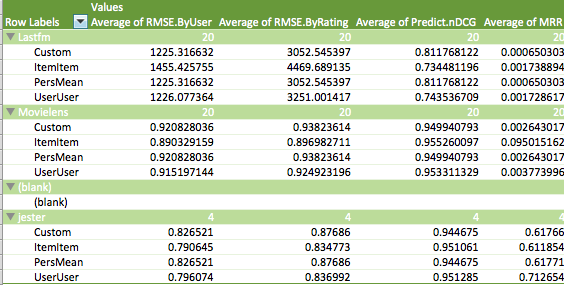
\includegraphics[scale=0.75]{Tabla.png}


\section{Datasets}
\subsection{LastFM}
\#Users: 1892 users \\
\#Items: 17632 artists \\
This dataset contains 92.834 user-artist relations. Each relation represents the number of times a user listened to an artist. In order to run the recommender system algorithms, we decided to consider this counter as a kind of rating.

\subsection{Movielens}
\#Users: 943 users \\
\#Items: 1682  movies \\
This dataset contains 100.000 user-movie relations. Each relation represents the evaluation of a movie by a user (in a scale from 1 to 5).

\subsection{Jester}
\#Users: 73.495 users \\
\#Items: 100 jokes \\
This dataset contains 4.1 million of user-joke relations. Each relation represents the evaluation of a movie by a user (in a scale from -10.0 to 10.0). As the scale is different to the used in Movielens, we decided to normalized the evaluations to a scale of [1,5]. Thus, the results of running the algorithm with Jester and Movielens can be comparable.

\subsection{Bookcrossing}
\#Users: 278.858 users \\
\#Items: 271.379 books \\
This dataset contains 1.149.780 of user-book relations. Each relation represents the evaluation of a book by a user. Also with this dataset, we normalized the ratings to a scale of [1,5].

\section{Metrics}
\subsection{RMSE}
RMSE reflects the difference between the real values and those predicted by the algorithm.
It is calculated in two ways:
\begin{itemize}
	\item Grouped by user: RMSE.byUser
	\begin{equation}
		\frac{\displaystyle\sum_{\forall\ user\ j}\sqrt{\frac{\displaystyle\sum_{\forall\ rating\ i} err_{ij}^2}{Total\ ratings\ user\ i}}}{Total\ users}
    \end{equation}
    \item Globally: RMSE.byRating 
	\begin{equation}
		\sqrt{\frac{\displaystyle\sum_{\forall\ user\ j}\displaystyle\sum_{\forall\ rating\ i} err_{ij}^2}{Total\ ratings}}
    \end{equation}
\end {itemize}

In general, both ways gives similar results.

In the case of LastFM, while grouping by users, the results are approximately a third of those obtained using the Global expression.

%Las medidas calculadas de ambas formas dan muy parecidas en general.
%Para el caso de lastfm la diferencia que calcula es de un tercio cuando se agrupa por usuario.
%Intentar entender esto: Pareciera que los usuarios se comportan muy diferente entre si pero no logro entender como.

\subsection{MRR}
This metric gives particular good results for Jester. That seems to be caused by the reduced number of items in the dataset (only 100 jokes). We could say that it is easier to "guess" the correct ranking in Jester than in the other datasets because of it has less items to order.
Also it's curious that MRR result for Movielens using CF item-item are approximately 40 times better than the outcome for the same metric, the same dataset, but with other algorithms.

%Performa especialmente bien para el caso de jester. Esto parece deberse a que la cantidad de items es mucho menor que para los otros casos (100)
%Es decir que es más simple poner un ranking correcto.

%Para el caso de movielens es inusualmente acertado con esta medida el itemitem por varias ordenes de magnitud (40 veces). Si bien la diferencia

\section{Algorithms}
\subsection{CF Item-item}
For the rating evaluations, is the algorithm with the best performance in Jester and Movielens. But with LastFm it is worse than CF User-user.


%Es el que mejor performa para los casos de rating: jester, movielens. 3% mejor
%Para el caso lastfm performa bastante peor: 29%






\end{document}